\documentclass{beamer}
\usepackage[utf8]{inputenc}
\usetheme{Madrid}
\usecolortheme{default}
\usepackage{amsmath,amssymb,amsfonts,amsthm}
\usepackage{txfonts}
\usepackage{tkz-euclide}
\usepackage{listings}
\usepackage{adjustbox}
\usepackage{array}
\usepackage{tabularx}
\usepackage{gvv}
\usepackage{lmodern}
\usepackage{circuitikz}
\usepackage{tikz}
\usepackage{graphicx}

\setbeamertemplate{page number in head/foot}[totalframenumber]

\usepackage{tcolorbox}
\tcbuselibrary{minted,breakable,xparse,skins}



\definecolor{bg}{gray}{0.95}
\DeclareTCBListing{mintedbox}{O{}m!O{}}{%
  breakable=true,
  listing engine=minted,
  listing only,
  minted language=#2,
  minted style=default,
  minted options={%
    linenos,
    gobble=0,
    breaklines=true,
    breakafter=,,
    fontsize=\small,
    numbersep=8pt,
    #1},
  boxsep=0pt,
  left skip=0pt,
  right skip=0pt,
  left=25pt,
  right=0pt,
  top=3pt,
  bottom=3pt,
  arc=5pt,
  leftrule=0pt,
  rightrule=0pt,
  bottomrule=2pt,
  toprule=2pt,
  colback=bg,
  colframe=orange!70,
  enhanced,
  overlay={%
    \begin{tcbclipinterior}
    \fill[orange!20!white] (frame.south west) rectangle ([xshift=20pt]frame.north west);
    \end{tcbclipinterior}},
  #3,
}
\lstset{
    language=C,
    basicstyle=\ttfamily\small,
    keywordstyle=\color{blue},
    stringstyle=\color{orange},
    commentstyle=\color{green!60!black},
    numbers=left,
    numberstyle=\tiny\color{gray},
    breaklines=true,
    showstringspaces=false,
}
%------------------------------------------------------------
%This block of code defines the information to appear in the
%Title page
\title %optional
{2.7.9}

%\subtitle{A short story}

\author % (optional)
{stalin-ai25btech11037}



\begin{document}


\frame{\titlepage}
\begin{frame}{Question}
Find the area of the triangle whose vertices are $P(1,0)$, $Q(2,2)$ and $R(3,1)$.\\ 
\end{frame}
\begin{frame}{Theoretical Solution}
Let us solve the given equation theoretically and then verify the solution computationally \\
According to the question, \\
Given three points\\
\begin{align}
  \vec{P}=\begin{myvec}{1\\0}\end{myvec}\;
  \vec{Q}=\begin{myvec}{2\\2}\end{myvec}\;
  \vec{R}=\begin{myvec}{3\\1}\end{myvec}\
   \end{align}
   \begin{align}
 \vec{Q}-\vec{P}=\begin{myvec}{1\\2}\end{myvec}\
\end{align}
\begin{align}
  \vec{R}-\vec{P}=\begin{myvec}{2\\1}\end{myvec}\
\end{align}
\begin{align}
ar(PQR) &= \frac{1}{2} \, \|(\vec{Q} - \vec{P}) \times (\vec{R} - \vec{P}) \|
\end{align}

\end{frame}
\begin{frame}{Theoretical Solution}
\begin{align}
ar(PQR) &= \frac{1}{2} \, \|(\vec{Q} - \vec{P}) \times (\vec{R} - \vec{P}) \|=\frac{3}{2}
\end{align}
\end{frame}
\begin{frame}[fragile]
    \frametitle{C Code}
    \begin{lstlisting}
#include <stdio.h>
#include <stdlib.h>

int main() {
    // Coordinates of the triangle
    int x1 = 1, y1 = 0;
    int x2 = 2, y2 = 2;
    int x3 = 3, y3 = 1;

    // Applying formula
    int determinant = x1*(y2 - y3) + x2*(y3 - y1) + x3*(y1 - y2);
    float area = 0.5 * abs(determinant);

    printf("Area of the triangle = %.2f\n", area);

    return 0;
}

     \end{lstlisting}
\end{frame}
\begin{frame}[fragile]
    \frametitle{python code }
    \begin{lstlisting}
import matplotlib.pyplot as plt
import numpy as np

# Vertices
P = np.array([1, 0])
Q = np.array([2, 2])
R = np.array([3, 1])

# Function to compute area using determinant formula
def triangle_area(A, B, C):
    return 0.5 * abs(A[0]*(B[1]-C[1]) + B[0]*(C[1]-A[1]) + C[0]*(A[1]-B[1]))

# Compute area
area = triangle_area(P, Q, R)
print("Area of triangle:", area)




    \end{lstlisting}
\end{frame}
\begin{frame}[fragile]
    \frametitle{python code }
    \begin{lstlisting}
# Plotting
x = [P[0], Q[0], R[0], P[0]]  # closing the triangle
y = [P[1], Q[1], R[1], P[1]]

plt.figure(figsize=(6,6))
plt.plot(x, y, 'b-o', linewidth=2)  # triangle edges
plt.fill(x, y, 'skyblue', alpha=0.5)  # fill triangle

# Mark vertices
plt.text(P[0], P[1]-0.2, "P(1,0)", fontsize=12, ha="center")
plt.text(Q[0], Q[1]+0.2, "Q(2,2)", fontsize=12, ha="center")
plt.text(R[0], R[1]-0.2, "R(3,1)", fontsize=12, ha="center")

\end{lstlisting}
\end{frame}
\begin{frame}[fragile]
    \frametitle{python code }
    \begin{lstlisting}
# Display area on plot
plt.title(f"Triangle PQR, Area = {area}")
plt.axis("equal")
plt.grid(True)

# Save figure
plt.savefig("triangle_area.png", dpi=300)
plt.show()
    \end{lstlisting}
\end{frame}
\begin{frame}{Plot}
    \centering
    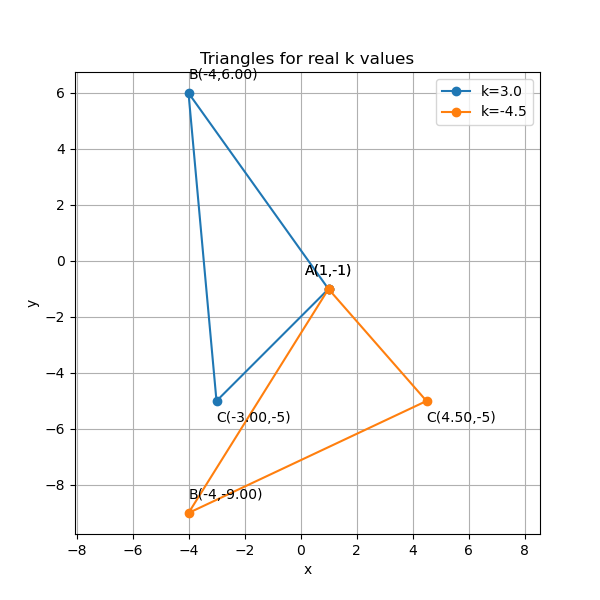
\includegraphics[width=\columnwidth, height=0.8\textheight, keepaspectratio]{figs/triangle_area.png}     
\end{frame}

\end{document}